\documentclass{beamer}

\usepackage[utf8]{inputenc}
\usepackage{pdfpages}
\usepackage{listings}


%Information to be included in the title page:
\title{Foreman Provisioning}
\author{Emerson Ford}
\date{}



\begin{document}
\frame{\titlepage}

\begin{frame}
	\frametitle{SLATE Provisioning Goals}
	\begin{itemize}
		\item Plug into existing infrastructure
		\item Solution should be adaptable to a variety of scenarios
		      \begin{itemize}
			      \item No network configuration access
			      \item Have network configuration access
		      \end{itemize}
		\item Majority of work is pushed to us, not to staff at remote site
		\item Provide plenty of automation opportunities
		\item Provide centralized reporting of hosts
		\item Scalable, both with the number of hosts and distances between hosts
		\item Could potentially plug into other cloud providers.
	\end{itemize}
\end{frame}

\begin{frame}[fragile]
	\frametitle{Overview of Provisioning}
	\begin{columns}
		\begin{column}{0.5\textwidth}
			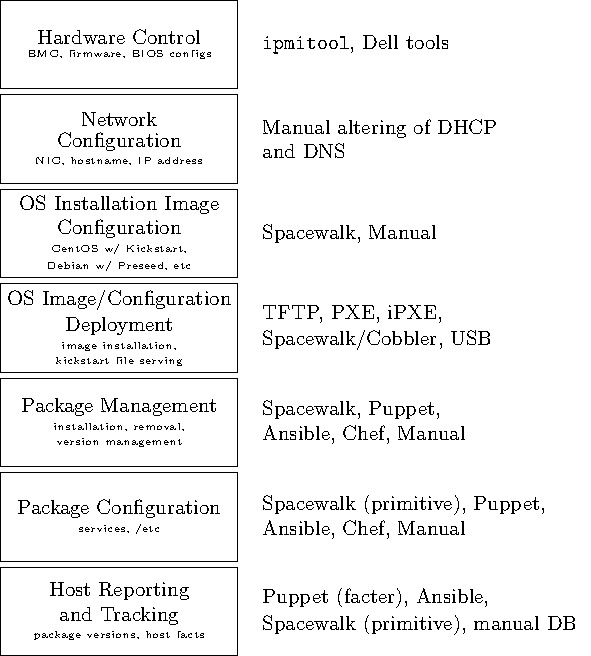
\includegraphics[width=\textwidth,height=\textheight-15mm,keepaspectratio]{provisioning_diagram}
		\end{column}

		\begin{column}{0.5\textwidth}
			Provisioning new machines is complicated... at the CHPC we have the following options:
			\begin{itemize}
				\item Can do all of this manually.
				\item Use Spacewalk, configure the rest manually.
				\item Configure hardware control \& network configuration manually, use one image/directory (through NFS) for all nodes (our compute nodes)
			\end{itemize}
			These aren't really scalable...
		\end{column}
	\end{columns}
\end{frame}

\begin{frame}
	\frametitle{What is Foreman?}
	An open-source project that acts as the "glue" between all of these pieces required for provisioning.
	It is extremely modular and plugs into existing projects like Puppet, xinetd, Kickstart, etc.
\end{frame}

\begin{frame}
	\frametitle{Foreman Architecture Overview}
	\begin{figure}[t]
		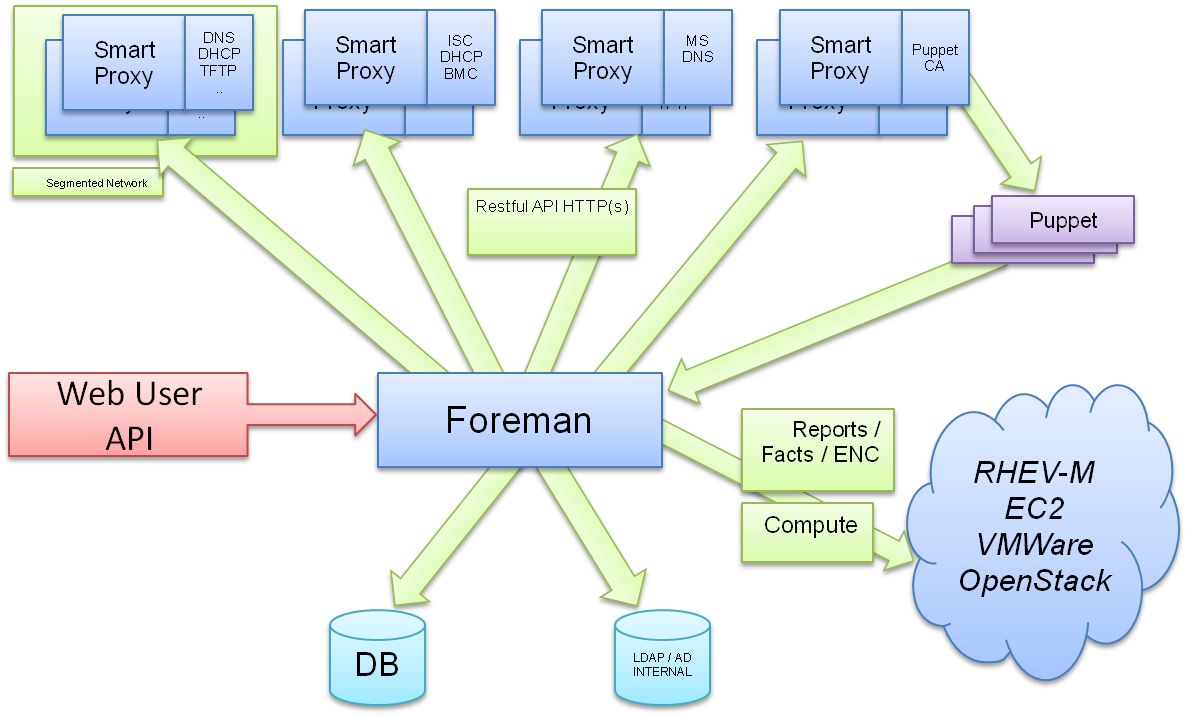
\includegraphics[width=\textwidth,height=\textheight-4cm,keepaspectratio]{foreman_architecture}

		\tiny Credit: Foreman Manual
		\vspace{0.1cm}

		\normalsize Each piece of Foreman can be deployed on individual servers. Smart Proxies plug into existing services, such as an already running \texttt{tftpd}.
	\end{figure}



\end{frame}

\begin{frame}
	\frametitle{Use Cases for Foreman}

\end{frame}

\begin{frame}[fragile]
	\frametitle{Custom iPXE Image}
	\flushleft
	Near vanilla iPXE image with the following embedded script:

	\centering
	\begin{lstlisting}[language=bash,frame=single,basicstyle=\fontsize{4}{6pt}\selectfont]
#!ipxe
# Intermediate iPXE script to report MAC address to Foreman

:net0
isset ${net0/mac} || goto no_nic
dhcp net0 || goto net1
chain http://fm-test.chpc.utah.edu/unattended/iPXE?mac=${net0/mac} || goto net1

:net1
isset ${net1/mac} || goto no_nic
dhcp net1 || goto net2
chain http://fm-test.chpc.utah.edu/unattended/iPXE?mac=${net1/mac} || goto net2

...


:net33
goto no_nic

exit 0

:no_nic
echo Failed to chainload from any network interface
sleep 30
exit 1
  \end{lstlisting}

\end{frame}

\begin{frame}[fragile]
	\frametitle{Foreman iPXE Workflow}

	\begin{columns}
		\begin{column}{0.5\textwidth}
			\flushleft
			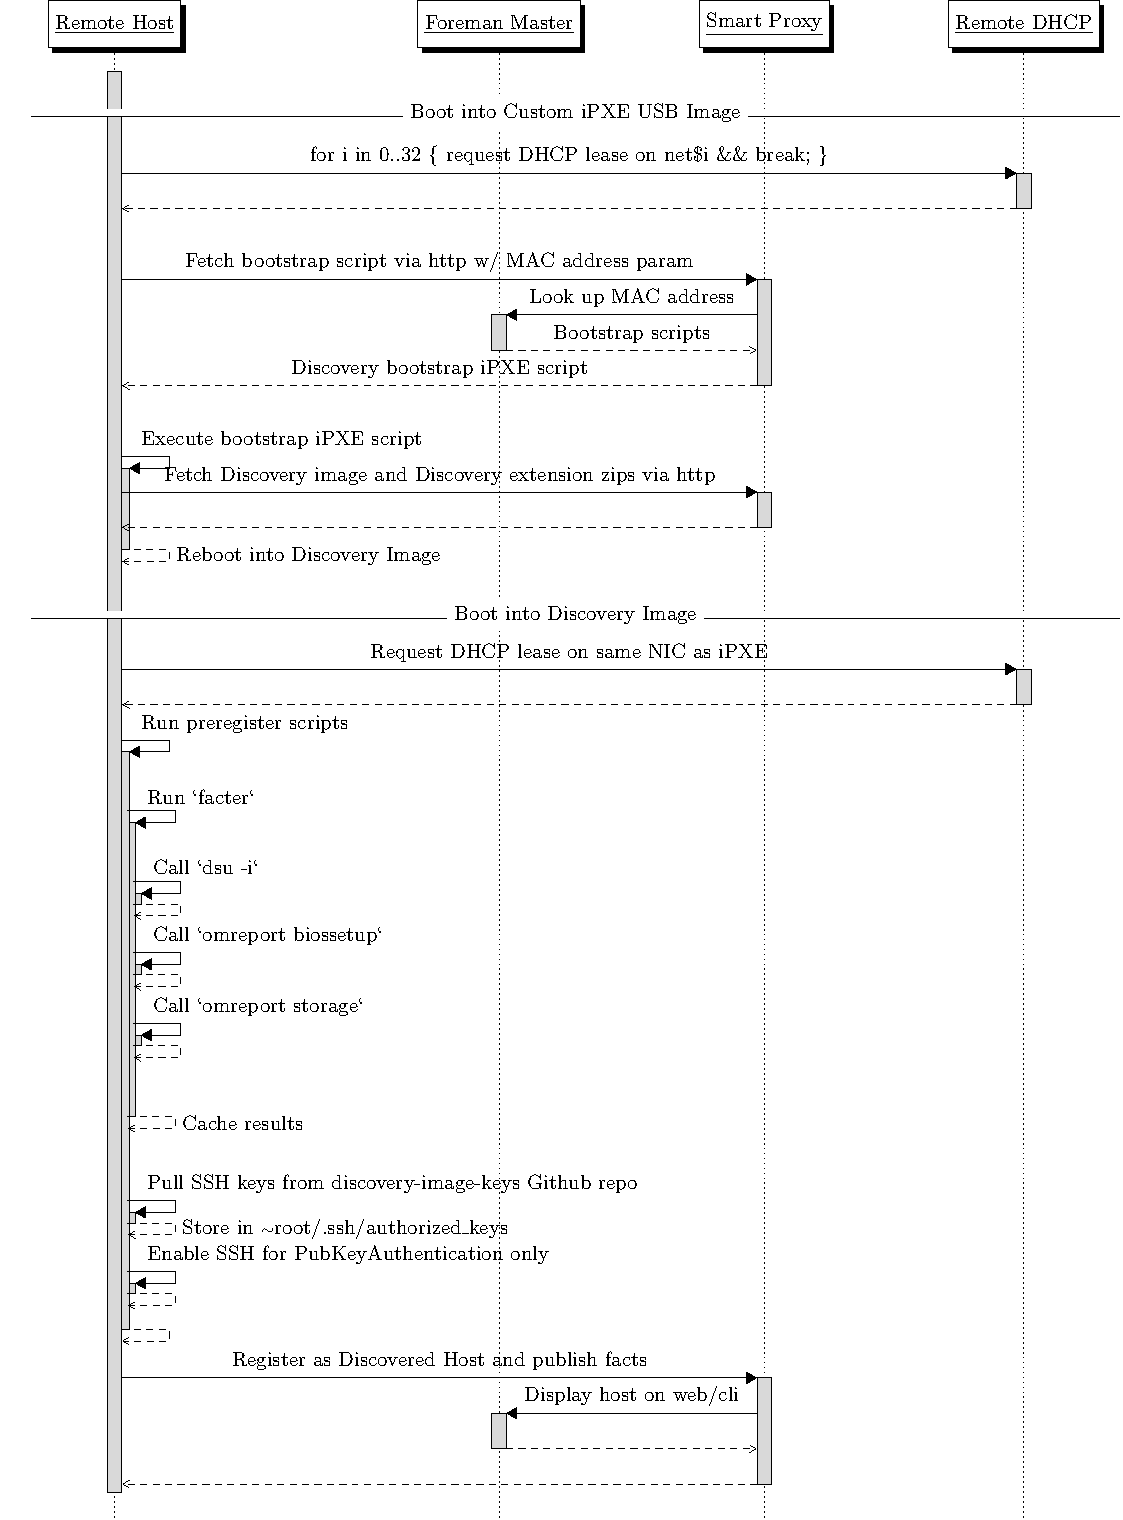
\includegraphics[width=\textwidth,height=\textheight-15mm,keepaspectratio]{discovery_sd}
		\end{column}

		\begin{column}{0.5\textwidth}
			Boot into Custom iPXE Image can happen in two ways:
			\begin{itemize}
				\item USB boot with custom iPXE image.
				\item PXE boot into custom iPXE image (configure DHCP):
				      \begin{lstlisting}[frame=single,basicstyle=\fontsize{3.5}{6pt}\selectfont]
if exists user-class and option user-class = "iPXE" {
  filename "http://fm-test.chpc.utah.edu/unattended/iPXE?bootstrap=1";
} elsif option architecture = 00:06 {
  filename "ipxe.efi";
} elsif option architecture = 00:07 {
  filename "ipxe.efi";
} elsif option architecture = 00:09 {
  filename "ipxe.efi";
} else {
  filename "undionly.0";
}
          \end{lstlisting}
			\end{itemize}
		\end{column}
	\end{columns}
\end{frame}

\begin{frame}[fragile]
	\frametitle{Foreman Installation Workflow}

	\centering
	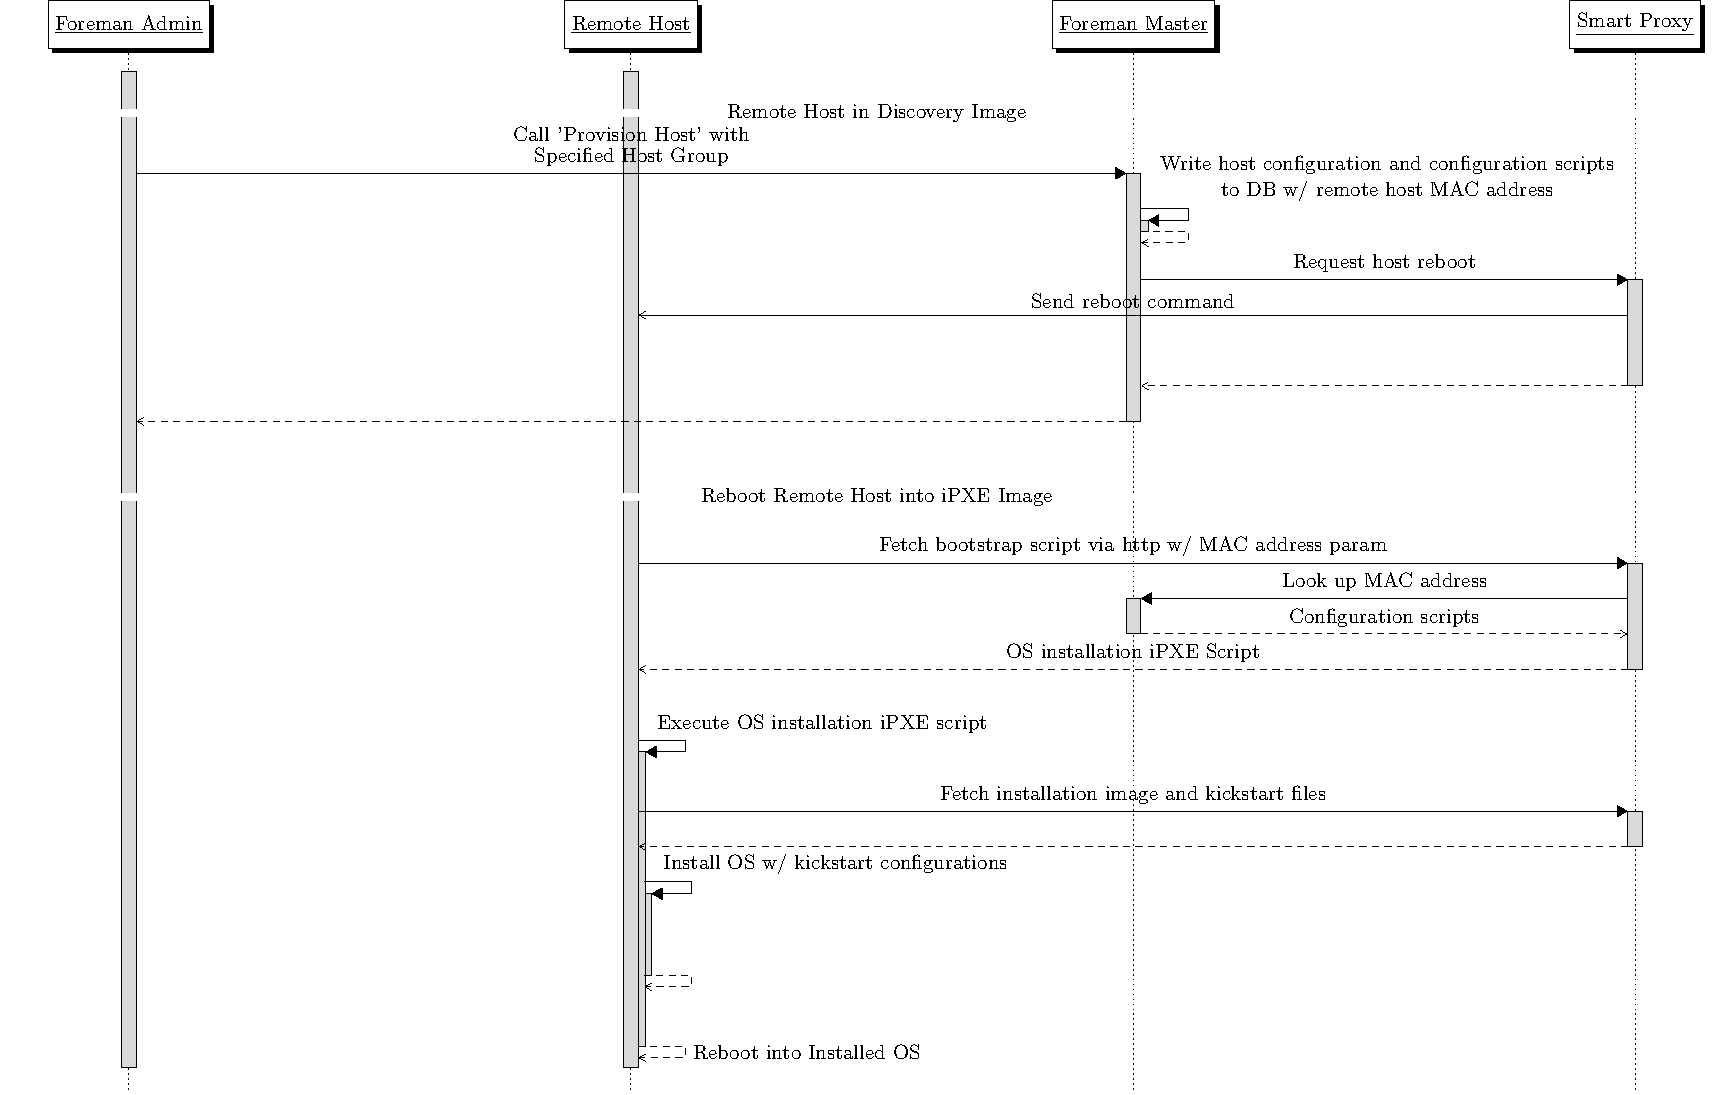
\includegraphics[width=\textwidth,height=\textheight-15mm,keepaspectratio]{installation_sd}
	\tiny
	Foreman supports kickstart files (RedHat), preseed files (Debian), etc.

\end{frame}

\begin{frame}[fragile]
	\frametitle{Foreman Configuration Workflow}

	\centering
	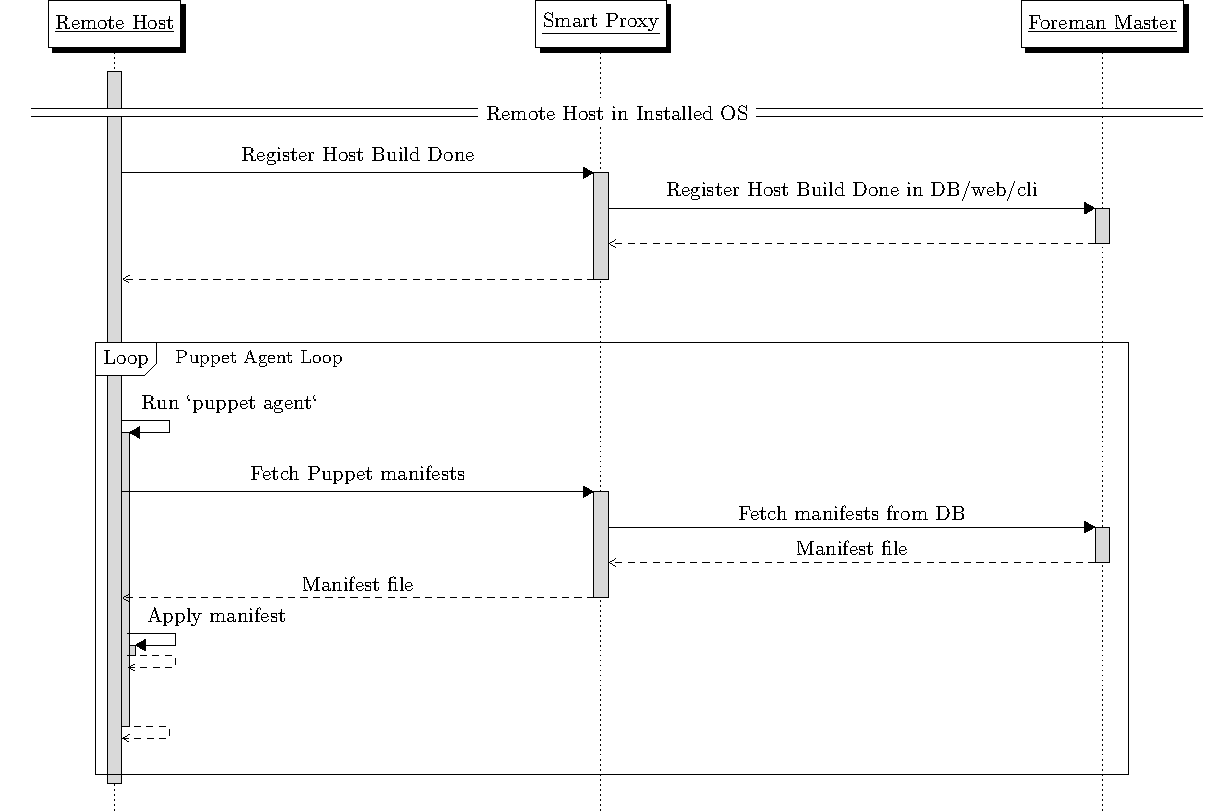
\includegraphics[width=\textwidth,height=\textheight-15mm,keepaspectratio]{configuration_sd}
	\tiny
	Foreman comes with Puppet by default but can be configured with Ansible, SaltStack, etc.

\end{frame}



\end{document}
